% Source: Lecture17_18.pdf, pages 4-11 (Lecture 18).
% Title on the source: "Lecture 18: RG and the epsilon expansion; epsilon = 4 - d".
\lecture{18}
\subsection{Momentum-space RG and the \texorpdfstring{$\epsilon$}{epsilon} expansion}
\subsubsection*{Momentum-space RG and field theory}

Our discussion follows the review by K.~Wilson and J.~Kogut, Physics Reports \textbf{12C}, 75 (1974),
section~4.2.

The real-space RG is equivalent, via a Fourier transformation from $\mathbf x\to\mathbf q$, to momentum
space; $q\leftrightarrow-\ii\partial/\partial x$, $\mathbf q\leftrightarrow-\ii\boldsymbol\nabla$. The
momentum-space RG is conventionally formulated by using field-theory methods. The Landau--Ginzburg free
energy for a bicritical point with zero external field, $H = 0$, for, say, an Ising model is
$A(T,H=0) = L_2M^2 + L_4M^4$, where $M = \ev{\sigma}$. One could add a kinetic term to this,
$\propto|\boldsymbol\nabla M|^2$, but this is zero when one is considering the ground state, as we did before,
since the state of minimum energy has $M$ = constant. The free energy has the invariance $M\to-M$,
corresponding to $\sigma\to-\sigma$. One can study a field theory of a real scalar field $\varphi$ described by
the path integral
\begin{equation}
  Z = \int\left[\prod_x\dd\varphi(x)\right]e^{\ii S},\qquad S = \int\dd^dx\,\mathcal L(\varphi,\partial_\mu\varphi),
\end{equation}
the ``action'' (take $\hbar = 1$ here), where $\mathcal L$ = Lagrangian density,
\begin{equation}
  \mathcal L = \frac{1}{2}(\partial_\mu\varphi)^2 - \frac{1}{2}\mu^2\varphi^2 - \frac{\lambda}{4}\varphi^4 .
\end{equation}
Make a Wick rotation to Euclidean metric, $\dd t\to-\ii\dd\tau$:
$(\partial_\mu\varphi)^2 = (\partial_t\varphi)^2-|\boldsymbol\nabla\varphi|^2\to-(\partial_i\varphi)^2$; thus
\begin{equation}
  \mathcal L_{\text{Euc}} = \frac{1}{2}(\partial_i\varphi)^2 + \frac{1}{2}\mu^2\varphi^2 + \frac{\lambda}{4}\varphi^4,
  \qquad Z = \int\left[\prod_x\dd\varphi(x)\right]e^{-S_{\text{Euc}}} .
\end{equation}
Denote $\lambda = u$. This has a $\mathbb{Z}_2$ invariance, the same as the Ising model. In
\begin{equation}
  Z = \int\dd^dx\left[\prod_x\dd\varphi(x)\,\delta(\varphi^2-c^2)\right]e^{-S_{\text{Euc}}},
\end{equation}
one reduces $\varphi$ to $\pm c$, i.e.\ to an Ising-type variable.

Dimensions: $S_{\text{Euc}}$ is dimensionless, so $\dd^dx\equiv\dd x_1\cdots\dd x_d$ has the dimension of
length$^d$ $\sim(1/\text{mass})^d$, so the mass dimension of $S_{\text{Euc}}$ is
\begin{equation}
  \dim(S_{\text{Euc}}) = 0 = -d + \dim\left((\partial_i\varphi)^2\right) = -d + 2 + 2\dim(\varphi),
\end{equation}
since $\dim\partial_i = 1$ $\Rightarrow\dim(\varphi) = (d-2)/2$ in mass units. Calculating the
dimension of the quartic coupling $u$ (called $\lambda$ in the quantum field theory literature and $u$ in the
statistical mechanics literature):
\begin{align}
  \dim(S_{\text{Euc}}) = 0 &= -d + \dim(u) + 4\dim(\varphi) = -d + \dim(u) + 4\left(\frac{d-2}{2}\right)\nonumber\\
  &= d-4+\dim(u)\ \Rightarrow\ \dim(u) = 4-d .
\end{align}
Now use integration by parts: $\dd(fg) = (\dd f)g + f(\dd g)\Rightarrow\int f\dd g = \int\dd(fg) - \int g\dd f$,
with $f = \partial_i\varphi$, $g = \partial_i\varphi$; the surface term $\to 0$, leaving $-\varphi\partial^2\varphi$,
where $\partial^2 = \sum_{i=1}^d\partial_i^2$. So the equivalent $\mathcal L$:
\begin{equation}
  S_{\text{Euc}} = \int\dd^dx\left[-\frac{1}{2}\varphi\,\partial^2\varphi + \frac{\mu^2}{2}\varphi^2 + u\varphi^4\right].
\end{equation}
($\mu^2$ is usually denoted $r$ in stat.\ mech.; don't confuse it with position $r$.) Under a Fourier
transform $-\ii\partial_j\to q_j$, $(-\ii\partial_j)(-\ii\partial_j) = -\partial^2\leftrightarrow\mathbf q^2$, where
$\mathbf q^2 = \sum_{j=1}^dq_j^2$. If $u = 0$, then
\begin{equation}
  S_{\text{Euc}} = \frac{1}{2}\int\dd^dx\,\varphi Q\varphi,\qquad Q = -\partial^2 + r = \mathbf q^2 + r,
\end{equation}
a quadratic integrand. So each functional integral is Gaussian (cf.\ $\int\dd x\,e^{-ax^2}$)
$\Rightarrow Q^{-1} = 1/(\mathbf q^2+r)$ plays the role of a ``propagator'' for the field $\varphi$ in a
diagrammatic perturbative expansion; the interaction is a vertex with four $\varphi$ lines and coupling $u$.

This is a continuum formulation: $\mathbf x$ and $\mathbf q$ are continuous variables. One formulates a
perturbative expansion around free field theory ($u = 0$).

\begin{diagram}
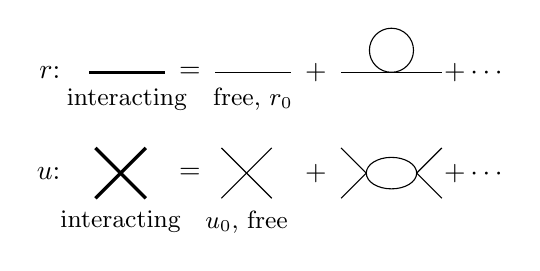
\begin{tikzpicture}[scale=0.8]
  \node[anchor=east] at (-0.3,0) {$r$:};
  \draw[very thick] (0,0) -- (1.2,0); \node[below,font=\small] at (0.6,-0.1) {interacting};
  \node at (1.6,0) {$=$};
  \draw (2,0) -- (3.2,0); \node[below,font=\small] at (2.6,-0.1) {free, $r_0$};
  \node at (3.6,0) {$+$};
  \draw (4,0) -- (5.6,0); \draw (4.8,0.35) circle (0.35);
  \node at (6.1,0) {$+\cdots$};
  \begin{scope}[yshift=-1.6cm]
  \node[anchor=east] at (-0.3,0) {$u$:};
  \draw[very thick] (0.1,-0.4) -- (0.9,0.4); \draw[very thick] (0.1,0.4) -- (0.9,-0.4);
  \node[below,font=\small] at (0.5,-0.45) {interacting};
  \node at (1.6,0) {$=$};
  \draw (2.1,-0.4) -- (2.9,0.4); \draw (2.1,0.4) -- (2.9,-0.4);
  \node[below,font=\small] at (2.5,-0.45) {$u_0$, free};
  \node at (3.6,0) {$+$};
  \draw (4,0.4) -- (4.4,0) -- (4,-0.4); \draw (5.6,0.4) -- (5.2,0) -- (5.6,-0.4);
  \draw (4.8,0) ellipse (0.4 and 0.25);
  \node at (6.1,0) {$+\cdots$};
  \end{scope}
\end{tikzpicture}
\diagramcaption{Perturbative corrections to $r$ and $u$.}
\end{diagram}

Higher-order terms induce changes in $r$ and $u$. The loops involve integrals over virtual momenta $\mathbf q$.
The analogue of the block-spin construction in real-space RG is integrating out the momenta above some scale
$\Lambda$, since large momenta are equivalent to short distances. The real-space RG flow on the couplings
$\{K_i\}$ in $\Ham$ is equivalent here to shifts in $r$ and $u$: $r\to r'$, $u\to u'$. One appeal of the
momentum-space RG is that one can formally generalize $d$ from a positive integer to a positive real number
and consider varying $d$. For a bicritical point, the dimension of $u$ plays an important role;
$\dim(u) = 4-d\equiv\epsilon$, so one can write
\begin{equation}
  u = \frac{\bar u}{\Lambda^{d-4}},
\end{equation}
where $\bar u$ is dimensionless and the dimensions of $u$ are explicitly embodied in $\Lambda$, and the
interaction term in $\mathcal L$ is then $(\bar u/\Lambda^{d-4})\varphi^4$, where $\Lambda$ is an ultraviolet
scale. For a continuous phase transition, we are interested in the long-distance behavior of the theory,
since the correlation length $\xi\to\infty$. This is the basis of the Kadanoff block-spin construction. In
momentum space this means that we are taking the infrared (IR) limit of the RG, integrating out the
short-distance, high-momentum effects. Equivalently, we are taking large $\Lambda$. So if $d>4$, the effect of
the interaction term $(\bar u/\Lambda^{d-4})\varphi^4\to 0$; it is an irrelevant operator in the RG
terminology. This means that the physics of the phase transition is that of a free-field theory
$\Leftrightarrow$ Gaussian integral, so the corresponding RGFP is called the Gaussian fixed point (GFP).
When $d<4$, then the $\varphi^4$ operator is relevant:
$u\varphi^4 = \bar u\Lambda^{4-d}\varphi^4 = \bar u\Lambda^\epsilon\varphi^4$, so this operator is a relevant
perturbation. Thus, the RG flow is such that:
\begin{itemize}
  \item $d>4\Rightarrow$ GFP is stable;
  \item $d<4\Rightarrow$ GFP is unstable, RG flow $\to$ the ``non-trivial'' fixed point.
\end{itemize}
One can study this behavior for small $\epsilon$, in terms of the ``$\epsilon$-expansion'', where
$\epsilon = 4-d$. With integration over high momenta corresponding to $b = 2$, the RG transformations on $r$ and
$u$ are displayed next. Further details are in J.~Kogut and K.G.~Wilson, Phys.\ Rept.\ \textbf{12}, 75 (1974).

\subsubsection*{The \texorpdfstring{$\epsilon$}{epsilon} expansion}

\begin{equation}
  r' = 4\left[r + \frac{3cu}{1+r}\right],\qquad
  u' = 2^\epsilon\left[u - \frac{9cu^2}{(1+r)^2}\right],
\end{equation}
where $\epsilon = 4-d$ and $c$ is a positive constant. Then
\begin{equation}
  M = \begin{pmatrix}\dfrac{\partial u'}{\partial u} & \dfrac{\partial u'}{\partial r}\\[6pt] \dfrac{\partial r'}{\partial u} & \dfrac{\partial r'}{\partial r}\end{pmatrix}
    = \begin{pmatrix}2^\epsilon\left[1-\dfrac{18cu}{(1+r)^2}\right] & \dfrac{18\cdot 2^\epsilon cu^2}{(1+r)^3}\\[12pt]
                     \dfrac{12c}{(1+r)} & 4\left[1-\dfrac{3cu}{(1+r)^2}\right]\end{pmatrix}.
\end{equation}

\paragraph{The Gaussian fixed point.} One of the RGFPs is the Gaussian fixed point (GFP):
$(u_*,r_*) = (0,0)$. (Recall that $r\sim L_2$ in the LG formalism, $r = L_2 = 0$ at $T = T_c$; the theory is
massless, $\mu = \xi^{-1} = 0$ in field theory terminology.) Then
\begin{equation}
  M_{\text{GFP}} = \begin{pmatrix}2^\epsilon & 0\\ 12c & 4\end{pmatrix},
\end{equation}
of triangular form, so
\begin{gather}
  \lambda_1 = 2^\epsilon = e^{\epsilon\ln 2} = 1+\epsilon\ln 2\ \text{for small }\epsilon,\quad
  \hat{\mathbf e}_1\propto\begin{pmatrix}1\\[6pt] \dfrac{12c}{-3+\epsilon\ln 2}\end{pmatrix}\simeq\begin{pmatrix}1\\ -4c\end{pmatrix};\nonumber\\
  \lambda_2 = 4,\quad \hat{\mathbf e}_2 = \begin{pmatrix}0\\1\end{pmatrix}.
\end{gather}
(In general: if $M = \left(\begin{smallmatrix}\lambda_1&0\\a&\lambda_2\end{smallmatrix}\right)$, then
$\hat{\mathbf e}_2 = \binom01$; $\hat{\mathbf e}_1\propto\binom{(\lambda_1-\lambda_2)/a}{1}\propto\binom{1}{a/(\lambda_1-\lambda_2)}$.)
\begin{itemize}
  \item If $d>4$, then $\epsilon<0$, so $\lambda_1<1$: the GFP is stable in the $\hat{\mathbf e}_1$ direction.
  \item If $d<4$, then $\epsilon>0$, so $\lambda_1>1$: the GFP is unstable in the $\hat{\mathbf e}_1$ direction.
  \item If $d = 4$, then $\epsilon = 0$, so $\lambda_1 = 1$; the $u$ parameter is marginal.
\end{itemize}
Since $\lambda_2>1$, the GFP is always unstable in the $\hat{\mathbf e}_2$ ($r$) direction. At the GFP,
$\lambda_2 = 4 = b^{y_2} = 2^{y_2}\Rightarrow y_2 = 2$ ($\hat{\mathbf e}_2\sim$ temperature direction $\sim r$
in LG), so $y_2 = y_\tau = 2\Rightarrow\nu = \nu' = 1/y_\tau = 1/2$, the MFT value.

\paragraph{The nontrivial fixed point.} The RG transformation has another RGFP at
\begin{equation}
  (u_*,r_*) = \left(\frac{\epsilon\ln 2}{9c},-\frac{4\epsilon\ln 2}{9}\right),
\end{equation}
called the ``nontrivial'' fixed point (NTFP) or Wilson--Fisher fixed point; consider this for small
$\epsilon$. Evaluating $M$ at this fixed point:
\begin{equation}
  M_{\text{NTFP}} = \begin{pmatrix}1-\epsilon\ln 2 & 0\\[6pt] 12c & 4\left(1-\dfrac{\epsilon\ln 2}{3}\right)\end{pmatrix},
  \qquad \lambda_1 = 1-\epsilon\ln 2 .
\end{equation}
If $d>4$, $\epsilon<0$, $\lambda_1>1$: the NTFP is unstable in the $\hat{\mathbf e}_1$ direction. If $d<4$,
$\epsilon>0$, $\lambda_1<1$: the NTFP is stable in the $\hat{\mathbf e}_1$ direction. $\lambda_2\simeq 4>1$, so the
NTFP is always unstable in the $\hat{\mathbf e}_2$ direction $=\hat{\mathbf e}_\tau$.

\begin{diagram}
\begin{tikzpicture}[scale=0.8,>=Stealth]
  \foreach \s/\lab/\nt in {0/{$d>4$, i.e.\ $\epsilon<0$}/1.6, 7.5/{$d<4$, i.e.\ $\epsilon>0$}/1.6} {
  \begin{scope}[xshift=\s cm]
    \draw[->] (-2.2,0) -- (3.2,0) node[right] {$u$};
    \draw[->] (0,-2.5) -- (0,2.5) node[above] {$r\sim\hat{\mathbf e}_2$};
    \draw (-2,1) -- (3,-1.5) node[right] {$\hat{\mathbf e}_1$};
    \coordinate (g) at (0,0); \coordinate (n) at (\nt,-0.8);
    \draw[->,thick] (n) -- (\nt,1.8); \draw[->,thick] (n) -- (\nt,-2.3);
    \draw[->,thick] (g) -- (0,1.8); \draw[->,thick] (g) -- (0,-2.3);
    \fill (g) circle (0.07); \fill (n) circle (0.07);
    \node[blue,font=\small] at (-0.7,-0.45) {GFP};
    \node[blue,font=\small] at (\nt+0.7,-0.4) {NTFP};
    \node[font=\small] at (0.5,-3.1) {\lab};
  \end{scope}}
  % flows along e1
  \draw[->,thick] (0.75,-0.37) -- (0.3,-0.15); \draw[->,thick] (0.85,-0.42) -- (1.3,-0.65);
  \draw[->,thick] (-1.5,0.75) -- (-0.8,0.4); \draw[->,thick] (2.6,-1.3) -- (2.0,-1.0);
  \begin{scope}[xshift=7.5cm]
  \draw[->,thick] (0.3,-0.15) -- (0.9,-0.45); \draw[->,thick] (-0.4,0.2) -- (-1.2,0.6);
  \draw[->,thick] (2.6,-1.3) -- (2.0,-1.0);
  \end{scope}
\end{tikzpicture}
\diagramcaption{RG flows near the Gaussian and nontrivial fixed points. For $d>4$ the GFP attracts along
$\hat{\mathbf e}_1$; for $d<4$ the NTFP does. Both are unstable along $\hat{\mathbf e}_2$.}
\end{diagram}

For $d>4$, the critical behavior is mean-field like: $\nu = \nu' = 1/y_\tau = 1/2$; $u\to 0$ at the
GFP, $\mathcal L\to\mathcal L_{\text{free field}}$, so $\eta = 0$, etc. Since $\mathcal L\to\mathcal L_{\text{free}}$,
with the interaction term $\to 0$, this fixed point is called ``trivial'', synonymous with ``Gaussian'' since the
functional integration can be done exactly as a Gaussian integral. The fluctuations that are neglected by MFT are
not important, so the MFT exponents describe the critical behavior. Recall these: $\alpha = 0$, $\beta = 1/2$,
$\gamma = 1$, $\nu = 1/2$, $\eta = 0$, $\delta = 3$; $y_\tau = 1/\nu = 2$,
$\beta\delta = y_h/y_\tau = 3/2\Rightarrow y_h = 3$. $d = 4$ is the upper critical dimension
$d_{u.c.}$ here, meaning the dimension above which the critical behavior is MF-like.

For $d<4$, the nontrivial fixed point is stable in the $\hat{\mathbf e}_1$ direction, since
$\lambda_1 = 1-\epsilon\ln 2<1$. Now
\begin{equation}
  \lambda_2 = 4\left(1-\frac{1}{3}\epsilon\ln 2\right) = b^{y_2} = 2^{y_2},
\end{equation}
so $\ln\lambda_2 = y_2\ln 2$, $y_2 = \ln\lambda_2/(\ln 2)$;
$\ln\lambda_2 = 2\ln 2 + \ln\left(1-(\epsilon/3)\ln 2\right)$; for $\epsilon\ll 1$,
$\ln\lambda_2\simeq 2\ln 2-(\epsilon/3)\ln 2$, so for small $\epsilon$,
\begin{equation}
  y_2\simeq 2-\frac{\epsilon}{3} = 2\left(1-\frac{\epsilon}{6}\right);\qquad
  \nu = \frac{1}{y_2} = \frac{1}{2\left(1-\frac{\epsilon}{6}\right)}\simeq\frac{1}{2}\left(1+\frac{\epsilon}{6}\right),\qquad
  \nu\simeq\frac{1}{2}+\frac{\epsilon}{12}+\Order(\epsilon^2),
\end{equation}
with $y_2 = y_\tau$ since $r\sim\hat{\mathbf e}_2\sim$ temperature-like parameter. Note that
$\nu = \nu_{\text{MFT}} = 1/2$ as $\epsilon\to 0$. Including an external magnetic field as we did for the 1D
Ising model, one can calculate $y_h$ at the NTFP:
\begin{equation}
  \boxed{y_h = 3-\frac{\epsilon}{2}+\Order(\epsilon^2)}.
\end{equation}
Again, as with
\begin{equation}
  \boxed{y_\tau = 2-\frac{\epsilon}{3}+\Order(\epsilon^2)},
\end{equation}
both reduce to the MFT values as $\epsilon\to 0$. We thus see how the thermal and magnetic exponents approach
their MFT values as $d\nearrow 4$, and for $d>4$, these stay at their MFT values because the Gaussian fixed point
is stable. Knowing $y_\tau$ and $y_h$, one can calculate all of the other critical exponents for this Ising
model: besides $\nu = \nu' = 1/2+\epsilon/12+\Order(\epsilon^2)$, one gets
\begin{gather}
  \alpha = \alpha' = 0+\frac{\epsilon}{6}+\Order(\epsilon^2),\qquad
  \beta = \frac{1}{2}-\frac{\epsilon}{6}+\Order(\epsilon^2),\qquad
  \gamma = \gamma' = 1+\frac{\epsilon}{6}+\Order(\epsilon^2),\nonumber\\
  \delta = 3+\epsilon+\Order(\epsilon^2),\qquad
  \eta = \underbrace{0}_{\text{MFT}}+0\cdot\epsilon+\Order(\epsilon^2)
\end{gather}
($\eta = 0\Leftrightarrow$ the free field has Maxwellian dimension, so
$\ev{\varphi_0\varphi_x}\sim1/x^{d-2+\eta}$, $\eta = 0$).

\paragraph{Comparison with series, experiment and exact results.}

Evaluating the $\Order(\epsilon)$ results for $\epsilon = 1$, i.e.\ $d = 3$:
\begin{center}
\renewcommand{\arraystretch}{1.2}
\begin{tabular}{lccc}
  & $\epsilon$ expansion, $d = 3$ & exp.--series & MFT\\ \hline
  $\alpha = \alpha'$ & $1/6 = 0.17$ & 0.11--0.12 & 0\\
  $\beta$ & $1/2-1/6 = 1/3 = 0.33$ & 0.325 & 0.5\\
  $\gamma = \gamma'$ & $1+1/6 = 7/6 = 1.17$ & 1.24 & 1\\
  $\nu = \nu'$ & $1/2+1/12 = 7/12 = 0.58$ & 0.63 & 0.5\\
  $\eta$ & $\simeq 0$ & 0.03 & 0\\
  $\delta$ & 4 & 4.8 & 3
\end{tabular}
\end{center}
So this RG calculation and $\epsilon$ expansion gives results that are closer to experiment than MFT, but the
results are not as accurate as series expansions.

Since $d = 2$, i.e.\ $\epsilon = 4-d = 2$, is farther from the expansion point, one does not expect the results
to be a very accurate description of the critical behavior in the 2D Ising model, and they are not:
\begin{center}
\renewcommand{\arraystretch}{1.2}
\begin{tabular}{lcc}
  & $\epsilon$ expansion, $d = 2$ & exact value\\ \hline
  $\alpha = \alpha'$ & $0+\epsilon/6 = 1/3 = 0.33$ & 0 (log div.)\\
  $\beta$ & $1/2-\epsilon/6 = 1/2-1/3 = 1/6 = 0.17$ & $1/8 = 0.125$\\
  $\gamma = \gamma'$ & $1+\epsilon/6 = 4/3 = 1.33$ & $7/4 = 1.75$\\
  $\nu = \nu'$ & $1/2+\epsilon/12 = 1/2+1/6 = 2/3 = 0.67$ & 1\\
  $\eta$ & $0+\Order(\epsilon^2)$ & $1/4 = 0.25$\\
  $\delta$ & $3+\epsilon = 5$ & 15
\end{tabular}
\end{center}
Although the RG and $\epsilon$ expansion below the $d_{u.c.} = 4$ is not as accurate in $d = 3$ as results from
series expansions, it does enable one to see how critical behavior changes as a function of dimension $d$ for
continuous $d$.

In contrast to high-temperature or low-temperature series, which are Taylor series expansions with finite radii
of convergence, the $\epsilon$ expansion has zero radius of convergence. Recall that a function $f(z)$ has a
Taylor series expansion at a point $z_0$,
\begin{equation}
  f(z) = f(z_0) + \sum_{n=1}^\infty\left(\frac{\dd^nf}{\dd z^n}\right)_{z_0}\frac{(z-z_0)^n}{n!},
\end{equation}
if it is analytic at $z_0$; physically this means that the properties of the function do not change abruptly at
$z_0$; one can analytically continue through this point smoothly. But this is not true at $\epsilon = 0$, because
the properties of the theory do change abruptly: for $\epsilon>0$, i.e.\ $d<4$, the NTFP is stable, but as $d$
increases through $d = 4$, i.e.\ $\epsilon$ decreases through 0, the GFP becomes stable and the critical behavior
changes to mean-field-like.

So in contrast to series calculations, one does not expect, in general, that calculating $y_\tau$, $y_h$, and the
other exponents to higher order in $\epsilon$ would necessarily improve the comparison with experiment/series
results in $d = 3$ and the exactly known results in $d = 2$. E.g.
\begin{equation}
  \gamma = 1+\frac{\epsilon}{6}+\frac{25}{324}\epsilon^2+\gamma_3\epsilon^3+\Order(\epsilon^4)
\end{equation}
$\Rightarrow$ for $d = 3$, $\gamma = 7/6 = 1.17$ to $\Order(\epsilon)$, $\gamma = 1.24$ to $\Order(\epsilon^2)$,
$\gamma = 1.195$ to $\Order(\epsilon^3)$, as compared with series and experiment $\gamma = 1.24$ for $d = 3$ Ising.
So, as illustrated by this calculation of $\gamma$ to $\Order(\epsilon^3)$, going from $\Order(\epsilon)$ to
$\Order(\epsilon^2)$ improves agreement with series--experiment but going from $\Order(\epsilon^2)$ to
$\Order(\epsilon^3)$ makes the agreement worse. For $\eta$: $\eta = 0+0\cdot\epsilon+\epsilon^2/54$, so for
$d = 3$, this gives $\eta = 0.0185$, vs.\ the series--experiment value $\eta = 0.03$.

This RG analysis and $\epsilon$ expansion have also been done for the $O(N)$ spin model, with
$\boldsymbol\varphi = (\varphi_1,\ldots,\varphi_N)$. For the same reason as before, namely the fact that the
dimension of the coefficient $L_4$ of the $|\mathbf M|^4$ term in the LG free energy, or $u$ of the quartic term
$u|\boldsymbol\varphi|^4$ in $\mathcal L$, is $d_u = 4-d$, $d = 4$ is again the upper critical dimensionality,
$d_{u.c.}$, so the RG flow diagram is the same as for the Ising $= O(1)$ model: the GFP is stable along
$\hat{\mathbf e}_1$ if $d>4$ and unstable if $d<4$, the NTFP is unstable along $\hat{\mathbf e}_1$ if $d>4$ and
stable if $d<4$, and they are both unstable along $\hat{\mathbf e}_2$.

\subsubsection*{Upper critical dimension and tricritical points}

The determination of the upper critical dimension $d_{u.c.}$ can be generalized. This is defined as the dimension
above which the GFP becomes stable and hence the critical behavior becomes mean-field like. In the framework of
$\mathcal L$, this occurs when the coefficient of the highest-power interaction term has a dimension that passes
through 0; for the bicritical point this is $\dim(u) = 4-d$, so for $d>4$, $u = \bar u/\Lambda^{d-4}$, and in the
IR limit, this UV scale suppresses the $u\varphi^4$ term so that it does not affect the physics.

Now let us consider a LG free energy with the highest-power term $u_p\varphi^p$, where $p$ is a general integer
$>2$ (the $p = 2$ term $r\varphi^2$ is part of the quadratic $\mathcal L\leftrightarrow$ Gaussian F.P.). Let us
calculate $\dim(u_p)$. Recall that $\dim(S = \text{action}) = 0$ and $\dim(\varphi) = (d-2)/2$; the
$u_p\varphi^p$ term contributes $\int\dd^dx\,u_p\varphi^p$ to the action, so
\begin{equation}
  0 = -d + \dim(u_p) + p\cdot\dim(\varphi) = -d + \dim(u_p) + p\left(\frac{d-2}{2}\right)
  \ \Rightarrow\ \dim(u_p) = d - p\left(\frac{d-2}{2}\right).
\end{equation}
Now solve the equation $\dim(u_p) = 0$ to get $d_{u.c.}$:
$\dim(u_p) = 0\Leftrightarrow d = p\left(d/2-1\right)\Rightarrow d\left(1-p/2\right) = -p\Rightarrow
d = d_{u.c.} = -p/\left(1-p/2\right) = 2p/(p-2)$:
\begin{equation}
  \boxed{d_{u.c.} = \frac{2p}{p-2}}\qquad
  \begin{array}{c|c} p & d_{u.c.}\\ \hline 3 & 6\\ 4 & 4\\ 6 & 3\end{array}
\end{equation}
Note the $p\leftrightarrow d_{u.c.}$ symmetry; this can be made manifest by re-expressing the equation for
$d_{u.c.}$:
\begin{equation}
  d_{u.c.} = \frac{2p}{p-2} = \frac{2}{1-\frac{2}{p}}\ \Rightarrow\ \frac{1}{d_{u.c.}} = \frac{1}{2}\left(1-\frac{2}{p}\right)
  \ \Rightarrow\ \boxed{2\left(\frac{1}{d_{u.c.}}+\frac{1}{p}\right) = 1}.
\end{equation}
In addition to $d_{u.c.} = 4$ for $\mathcal L = (1/2)(\partial\varphi)^2 + r\varphi^2 + u_4\varphi^4$, we have
$d_{u.c.} = 3$ for
\begin{equation}
  \mathcal L = \frac{1}{2}(\partial\varphi)^2 + r\varphi^2 + u_4\varphi^4 + u_6\varphi^6 .
\end{equation}
This $\mathcal L$ has been used to describe a tricritical point, i.e.\ a phase transition such that one must tune
three relevant physical parameters to get to the critical point, as contrasted with two for a bicritical point
(temperature $T = T_c$ and external magnetic field $H = H_c = 0$, or $T = T_c$ and pressure $p = p_c$ for a
liquid--gas critical point).

An example of a tricritical point occurs in, e.g., an Ising antiferromagnet in $d = 2$ or 3 on a bipartite
lattice (square, sc, or bcc), with an external uniform magnetic field, $H$ (e.g.\ FeCl$_2$). The AFM spin--spin
interaction leads to a SSB with nonzero staggered (= sublattice) magnetization, i.e.\ AFM LRO. This is a
situation with competing interactions, since the
$-J\sum_{e_{ij}}\sigma_i\sigma_j = +|J|\sum_{e_{ij}}\sigma_i\sigma_j$ interaction favors AFM order, while the
$-H\sum_i\sigma_i$ interaction favors FM order. Here the relevant parameter would be a (hypothetical) staggered
magnetic field, $H_{st}$, which is taken to be zero.

\begin{diagram}
\begin{tikzpicture}[scale=0.9,>=Stealth]
  \draw[->] (0,0) -- (4.5,0) node[right] {$T$};
  \draw[->] (0,0) -- (0,4) node[above] {$H$};
  \draw[->] (0,0) -- (-1.6,-1.6) node[below left] {$H_{st}$};
  \draw[thick,blue] (3,0) .. controls (3,0.8) and (2.9,1.4) .. (2.5,1.9);
  \draw[thick,blue] (2.5,1.9) .. controls (2.3,2.5) and (2.2,3.0) .. (1.9,3.6);
  \draw[thick,blue] (2.5,1.9) .. controls (2.6,2.6) and (2.8,3.1) .. (3.0,3.6);
  \draw (0,2.6) .. controls (1,2.8) and (2,2.4) .. (2.5,1.9);
  \fill[red] (2.5,1.9) circle (0.07);
  \fill[blue] (3,0) circle (0.06);
  \node[below] at (3,0) {$T_c$};
  \node[red,anchor=west,font=\small] at (2.65,1.75) {tricritical pt.};
  \node[blue,anchor=west,font=\small,align=left] at (3.1,0.8) {line (curve) of\\ critical pts.};
  \node[anchor=east,font=\small,align=right] at (-0.2,3.2) {surfaces of 1st-order\\ phase transitions};
  \node[anchor=south west,font=\small,align=left] at (2.6,3.9) {1st-order curve,\\ 3-phase coexistence curve};
  \begin{scope}[xshift=9.3cm,yshift=0.8cm]
    \draw (0,0) rectangle (3,2.4); \draw (0,1.2) -- (3,1.2); \draw (1.5,0) -- (1.5,2.4);
    \draw[green!60!black,thick] (0,0.05) .. controls (1.3,0.1) and (1.45,0.4) .. (1.5,1.2) .. controls (1.55,2.0) and (1.7,2.3) .. (3,2.35);
    \draw[green!60!black,thick] (0,0.1) .. controls (1.1,0.25) and (1.35,0.6) .. (1.5,1.2) .. controls (1.65,1.8) and (1.9,2.15) .. (3,2.3);
    \draw[green!60!black,thick] (0,0.2) .. controls (0.9,0.4) and (1.25,0.8) .. (1.5,1.2) .. controls (1.75,1.6) and (2.1,2.0) .. (3,2.2);
    \node[left,font=\small] at (0,1.2) {$M_{st}$};
    \node[below,font=\small] at (1.5,0) {$H_{st}$};
    \node[green!60!black,font=\small,align=center] at (1.5,3.1) {$T<T_c$, $T = T_c$,\\ $T>T_c$};
  \end{scope}
\end{tikzpicture}
\diagramcaption{Phase diagram of an Ising antiferromagnet in a uniform field near a tricritical point (left).
At the tricritical point three ``lines'' (actually curves) of critical points meet, and three 1st-order surfaces
meet at the 1st-order 3-phase coexistence curve. Right: staggered magnetization as a function of the staggered
field.}
\end{diagram}

At the tricritical point, 3 ``lines'' (actually curves) of critical points meet, and one must tune three relevant
physical parameters to get the tricritical behavior: $T$, $H_{st}$, and $H$. The critical singularities depend on
the direction of approach to the tricritical point. The first-order transitions are embodied in a LG free energy
with $M^2$, $M^4$, and $M^6$ terms. The relative sizes of the coefficients $r$ of $M^2$ and $u_4$ of $M^4$ depend
on how one approaches the tricritical point:
\begin{equation}
  A = rM_{st}^2 + u_4M_{st}^4 + u_6M_{st}^6 ;
\end{equation}
depending on the parameters, this can produce a first-order transition or a second-order one.

\begin{diagram}
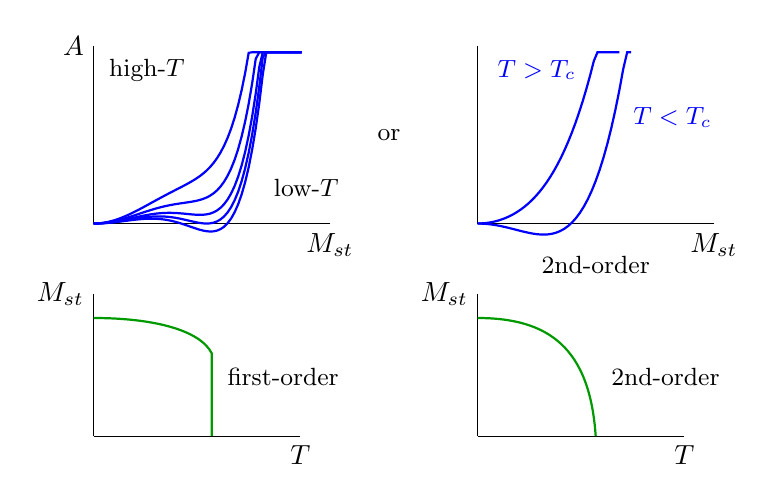
\begin{tikzpicture}[scale=0.75]
  \draw (0,0) -- (4,0) node[below] {$M_{st}$}; \draw (0,0) -- (0,3) node[left] {$A$};
  \foreach \a in {1.5,1.1,0.85,0.714,0.6} \draw[blue,thick,domain=0:2.2,samples=60] plot ({1.6*\x},{min(2.9,0.8*(\a*\x*\x-\x^4+0.35*\x^6))});
  \node[font=\small] at (0.9,2.6) {high-$T$}; \node[font=\small] at (3.6,0.6) {low-$T$};
  \node[font=\small] at (5,1.5) {or};
  \begin{scope}[xshift=6.5cm]
  \draw (0,0) -- (4,0) node[below] {$M_{st}$}; \draw (0,0) -- (0,3);
  \draw[blue,thick,domain=0:2.4,samples=40] plot (\x,{min(2.9,0.4*\x*\x+0.08*\x^4)});
  \draw[blue,thick,domain=0:2.6,samples=40] plot (\x,{min(2.9,-0.3*\x*\x+0.12*\x^4)});
  \node[blue,font=\small] at (1.0,2.6) {$T>T_c$}; \node[blue,font=\small] at (3.3,1.8) {$T<T_c$};
  \node[font=\small] at (2,-0.7) {2nd-order};
  \end{scope}
  \begin{scope}[yshift=-3.6cm]
  \draw (0,0) -- (3.5,0) node[below] {$T$}; \draw (0,0) -- (0,2.4) node[left] {$M_{st}$};
  \draw[green!60!black,thick] (0,2) .. controls (1,2) and (1.8,1.8) .. (2,1.4) -- (2,0);
  \node[anchor=west,font=\small] at (2.1,1.0) {first-order};
  \begin{scope}[xshift=6.5cm]
  \draw (0,0) -- (3.5,0) node[below] {$T$}; \draw (0,0) -- (0,2.4) node[left] {$M_{st}$};
  \draw[green!60!black,thick] (0,2) .. controls (1.2,2) and (1.9,1.5) .. (2,0);
  \node[anchor=west,font=\small] at (2.1,1.0) {2nd-order};
  \end{scope}
  \end{scope}
\end{tikzpicture}
\diagramcaption{Free energy with $M^2$, $M^4$, $M^6$ terms and the resulting first-order or second-order
behavior of the staggered magnetization.}
\end{diagram}

Since $\mathcal L\supset\varphi^6$ term, $d_{u.c.} = 3$ for a tricritical point. One interesting feature of
tricritical points is that this upper critical dimension is reached in physical systems; $d = 3$ is the usual
spatial dimension. Further details are e.g.\ in Plischke--Bergersen, 3rd ed., and Lawrie and Sarbach, vol.~9 of
Domb and Lebowitz, \emph{Phase Transitions and Critical Phenomena}.

Helmholtz free energy:
\begin{equation}
  A = c_2M^2 + c_4M^4 + c_6M^6;\qquad \left(\pder{A}{M}\right)_T = H,
\end{equation}
with $c_6>0$ for boundedness of the energy, and
\begin{equation}
  \pder{A}{M} = 2c_2M + 4c_4M^3 + 6c_6M^5 = 2M(c_2 + 2c_4M^2 + 3c_6M^4).
\end{equation}
Here $c_2\propto(T-T_t)+\cdots$; if $c_4/c_2\to 0$ at $T_t$ (e.g.\ for a suitable approach), then
\begin{equation}
  M^4 = -\frac{c_2}{3c_6}\propto(T_c-T)\ \Rightarrow\ M\sim|T_c-T|^{1/4},\qquad\beta = \frac{1}{4} .
\end{equation}

\paragraph{Lower critical dimension.}

In addition to $\epsilon$ expansions below $d_{u.c.}$, one can also calculate $\epsilon$ expansions above
$d_{\ell.c.}$ = lower critical dimensionality: $d_{\ell.c.} = 1$ for a discrete spin model, $d_{\ell.c.} = 2$ for
the $O(N)$ model with $N\ge 3$. So here $\epsilon = d-d_{\ell.c.}$. For the $2+\epsilon$ expansion of the $O(N)$
spin model, with an exact solution for $N\to\infty$, see
\begin{itemize}
  \item W.~Bardeen, B.W.~Lee, and R.~Shrock, Phys.\ Rev.\ D \textbf{14}, 985 (1976);
  \item E.~Br\'ezin, J.C.~Le~Guillou, and J.~Zinn-Justin, Phys.\ Rev.\ B \textbf{14}, 2615, 3110 (1976);
\end{itemize}
with
\begin{equation}
  \kB T_c = \frac{2\pi(d-2)}{N}.
\end{equation}
